% !TeX encoding = UTF-8

\documentclass{LTHtwocol} % Use this when you work on your report.
% \documentclass[final]{LTHtwocol} % Use this for the final version.
                                   % It will remove page numbers and
                                   % markers for overfull boxes.
                                   % There really shouldn't be any of those anyway.

\usepackage[utf8]{inputenc}
\usepackage{amsmath,amssymb,graphicx}
\usepackage{float}
\usepackage{xcolor}
\usepackage{hyperref}
\usepackage{algorithm}
\usepackage{algpseudocode}
\hypersetup{
	colorlinks,
	linkcolor={red!50!black},
	citecolor={blue!50!black},
	urlcolor={blue!80!black}
}

\usepackage{kantlipsum} % Only for the dummy text. Remove for your own report.

\addbibresource{bibliography.bib}

% Custom commands
% From: https://tex.stackexchange.com/questions/130307/questions-about-algpseudocode
\algnewcommand\True{\textbf{true}\space}
\algnewcommand\False{\textbf{false}\space}

% Document begins here
\begin{document}
\begin{frontmatter}
\title{Balance Double Inverted Pendulum on Cart} % Title of the project.
                      							 % Note that all reports are in English,
							                     %so that our international students can read them.

\author[cem]{Cem Alpt\"urk}
\author[pukashawar]{Pukashawar Pannu}

\email[cem]{ce5368al-s@student.lu.se}
\email[pukashawar]{pu6218pa-s@student.lu.se}

\begin{abstract}
    The abstract should be a 200--250 word compact description of your project. What was the objective? Which methods did you use? What was the (main) result?
\end{abstract}

\end{frontmatter}

% Stick to the proposed structure below. Add \subsections{} as appropriate.
% This file compiles on the Automatic Control Department system by typing the
% following into the terminal (while in the directory of the file, and with all
% other files belonging to the template untouched):
% > pdflatex template
% > biber template
% The first line compiles the .tex file. The second line generates the
% bibliography. Once this is done, you may need to run the first line 1-2
% additional times, for the system to get all cross references right in the
% produced pdf output.

\section{Introduction}
The goal of this project is to teach an agent to control a double pendulum on a cart to be standing upright, in its equilibrium point, using reinforcement learning.
A double pendulum is a highly chaotic system, where its behavior heavily depends on its initial conditions.
As a result, this system can be very difficult to control.
Figure \ref{fig:double_pendulum_chaotic} shows a simulation with 4 double pendulums with nearly identical initial conditions.
After some time their behaviors become so different that it becomes nearly impossible to make a prediction about the future.
This illustrates the chaotic behavior of this system.
Our aim is to create an agent that can learn from its own experiences to control the double pendulum, by applying a force on the cart in the horizontal direction, such that it stays upright.
Although this is an academic problem, the results could be applied to any type of learning problem since the agent is unaware of what it's working on.
(Possible reference to qlearning)
\begin{figure}[H]
	\centering
	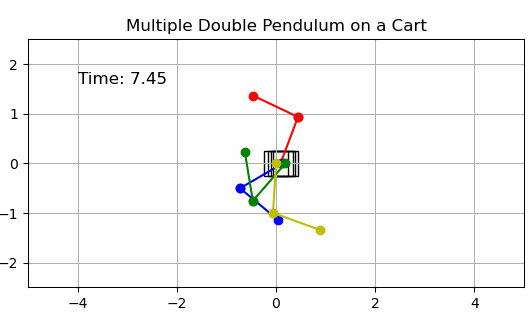
\includegraphics[width=0.9\columnwidth]{figures/Double_Pendulum_Chaotic.PNG}
	\label{fig:double_pendulum_chaotic}
	\caption{4 double pendulums simulated with similar initial conditions after $9.86$ seconds, with a difference of $0.02 rad/s$ differences on the inner pendulum angular velocities. All other initial states were equal.}
\end{figure}
% Here you introduce the project. What is the background? What project do you aim at solve? References to prior work? If the project makes a positive or negative environmental, or other solitary, impact, describe it here. Are there any ethical considerations? You might want to reference relevant literature, e.g. \cite{openclosed2, Hellerstein2004, Yun2015}. A general \LaTeX\ guide is available at \cite{latexwiki}.

\subsection{Reinforcement Learning}
%\kant[1] % This generates the dummy text
The main idea of reinforcement learning is to learn to make decisions based on past experiences.
In this case this means to train an agent that performs the best action, the force applied in the horizontal direction,  possible given the current states of the system.
For each action taken by the agent, the environment returns a new state and a reward for that action.
The reward is calculated based on how close the system is to its equilibrium point.
The goal of training the agent is to optimize gained reward for each action taken.

\section{Modeling}
The system consists of a cart that can move in the horizontal direction and two pendulums that are coupled to each other such that there is no collision between any parts.
Since this project is not about modeling the double pendulum, but rather about controlling it, we have borrowed the equations of motion from (ref).
The states of the system are represented by,
\begin{equation}
x  :=
\begin{bmatrix}
y & \dot{y}
\end{bmatrix}
^T , \quad y :=
\begin{bmatrix}
q & \theta_1 & \theta_2
\end{bmatrix}
^T
\end{equation}
%\begin{equation}
%x :=
%\begin{bmatrix}
%q & \theta_1 &  \theta_2 &  \dot{q} &  \dot{\theta_1} & \dot{\theta_2}
%\end{bmatrix}
% ^T
%\end{equation}
\begin{itemize}
\item $q$ is the position of the cart on the horizontal axis.
\item $\theta_1$ is the angle of the inner pendulum with respect to the vertical axis in the clockwise direction.
\item $\theta_2$ is the angle of the outer pendulum with respect to the vertical axis in the clockwise direction.
\item $\dot{q}$ is the velocity of the cart in the horizontal axis.
\item $\dot{\theta_1}$ is the angular velocity of the inner pendulum.
\item $\dot{\theta_2}$ is the angular velocity of the outer pendulum.
\end{itemize}

The system parameters are represented by,
\begin{itemize}
\item $m = 1 [kg]$ is the mass of the cart.
\item $m_1 = 0.1 [kg]$ is the mass of the inner pendulum.
\item $m_2 = 0.1[kg]$ is the mass of the outer pendulum.
\item $l_1 = 1 [m]$ is the length of the inner pendulum.
\item $l_2 = 1[m]$ is the length of the outer pendulum.
\item $g = 9.81 [m/s^2]$ is the gravitational acceleration.
 \end{itemize}

The equations of motions for this system (ref), are adjusted such there is no friction or disturbances.
The input to the system is a horizontal force that is acting on the cart, represented by $u$ $[N]$.

\begin{equation}
M(y) \ddot{y} = f(y,\dot{y},u)
\end{equation}


\begin{equation}
\resizebox{ \columnwidth}{!}
{
$
M(y) :=
\begin{bmatrix}
m + m_1 +m_2 & l_1(m_1+m_2)\cos \theta_1 & m_2 l_2 \cos \theta_2 \\
l_1 (m_1 + m_2) \cos \theta_1 & l_1^2(m_1+m_2) & l_1 l_2 m_2 \cos(\theta_1 - \theta_2) \\
l_2 m_2 \cos \theta_2 & l_1 l_2 m_2 \cos (\theta_1 - \theta_2) & l_2^2 m_2
\end{bmatrix}
$
}
\end{equation}

\begin{equation}
\resizebox{ \columnwidth}{!}
{
$
f(y,\dot{y},u) :=
\begin{bmatrix}
l_1(m_1+m_2) (\dot{\theta_1})^2 \sin \theta_1 + m_2 l_2 (\dot{\theta_2})^2 \sin \theta_2 + u\\
-l_1l_2m_2(\dot{\theta_2})^2 \sin(\theta_1 - \theta_2) + g(m_1 + m_2)l_1 \sin \theta_1 \\
l_1l_2m_2(\dot{\theta_1})^2 \sin (\theta_1 - \theta_2) + g l_2 m_2 \sin \theta_2
\end{bmatrix}
 $
 }
\end{equation}






%Here you present the modeling approach and publish your model. If your model has 63434 parameters, you may not wish to print it in detail. The idea is, however, that another group with your background should be able to reproduce your work -- this goes not only for the modeling aspect.
%
%If you use equations, make sure they are all numbered:
%\begin{equation}
%\alpha_a^2 + \beta_b^2 = \gamma_c^2.
%\label{eq:formula}
%\end{equation}
%Equations are parts of the text. If they end a sentence, they should end with a dot. If they end a clause, they should end with a comma. You refer to an equation this like: see \eqref{eq:formula}. Note that all units are written in roman type: $\omega=2\pi$~rad/s, $g = 9.81$~m/s$^2$. See \cite{mathslatexwiki} for a tutorial on typesetting maths.
%
%\subsection{Some Dummy Text}
%\kant[2]

\section{System Design}
A couple of reinforcement learning methods are Q-learning and Deep Q-learning.
\subsection{Q-learning}
Q-learning is a model free method where the agent has no information about the system its trying to control, thus it can be said that it is a black box model.
The agent stores all its experiences in a Q-table that contains the quality of a state-action combination.
\[ Q : S \times A  \to \mathbb{R} \]
\[Q(s,a) := \text{Quality of action $a$ given state  $s$} \]
A trained agent decides on the action to perform by looking up the best action $a$ given state $s$ from the Q-table.
In the case where multiple actions give the same values in the Q-table, the action is selected randomly among those.
The selected action is performed on the environment, which is the inverted pendulum, and a reward is calculated based on the new state of the system.
In the case where there is no previous knowledge about the current state in the Q-table, the action is selected randomly.
Essentially the agent tries to find the action that will give the best reward.
\[ a^* = \max_i Q(s,a_i) \]
Training the agent corresponds to populating and updating the Q-table based on past experiences of the agent.
After performing an action given the current state of the system, the agent receives a reward from the environment and the values in the Q-table are updated according to the state-action combination and the reward received.
\begin{equation}
Q^{new}(s_t,a_t) \leftarrow (1 - \alpha)Q(s_t,a_t) + \alpha (r_t + \gamma \max_i Q(s_{t+1},a_i ))
\label{eq:qlearning}
\end{equation}
\[ 0 < \alpha \leq 1, \quad 0 \leq \gamma \leq 1  \]
\[ Q(s_t,a_t) = E[r_t + \gamma r_{t+1} + \gamma^2 r_{t+2} + \hdots | s_t,a_t] \]
After performing action $a_t$ given the state $s_t$, the agent receives the new state $s_{t+1}$ and the reward $r_t$. The value $Q(s_t,a_t)$ is updated by \eqref{eq:qlearning}. $\alpha$ is the learning rate and $\gamma$ is the discount factor. Since the reward for a certain action might not come instantly, the discount factor tries to compensate for the delayed reward by estimating the reward that the agent will receive if it takes the best action $a_{t+1}$ for the state $s_{t+1}$. Low values of $\gamma$ will cause the agent to only consider near future rewards, while a $\gamma$ value close to 1 will consider

This method requires a discrete set of actions and states. For the double pendulum problem, this can be achieved by discretizing the states and actions.
However since this is a chaotic system, it would require a fine discretization resulting in a massive Q-table. Although this can work in theory, there are practical implementation limitations such as limited memory size.
This problem can be resolved by using the Deep Q-learning method.

\subsection{Deep Q-learning}
In Deep Q-learning, the Q-table is replaced with a deep neural network that tries to learn Q-values instead of memorizing them.
A benefit of using Deep Q-learning is that is uses less memory and it has more predictive power on unseen states.
The network takes in the system states as input arguments and predicts the q-values.
\begin{equation}
	\label{eqn:neural_network_mapping}
	NN_Q := \mathbb{R}^m \to \mathbb{R}^n
\end{equation}
where $m$ is the state size and $n$ is the size of the action space.
The agent chooses the action to perform by picking the largest q-value from the neural network prediction.
\begin{figure}[H]
	\centering
	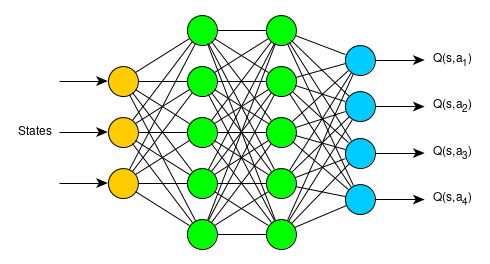
\includegraphics[width=0.9\columnwidth]{figures/q_network.png}
	\label{fig:q_network_illustration}
	\caption{Illustration of a neural network with $3$ inputs and $4$ outputs.}
\end{figure}


The neural network is trained by a method called experience replay that is based on simulating the system and recording all states, rewards and actions taken in memory.
The simulation ends when it reaches a termination condition that is defined in the environment.
For the double pendulum case the termination condition is when the outer pendulum angle becomes larger than a defined maximum value.
One full simulation from start to termination is called an episode.
The stored experience is used to fit the neural network once there is enough experience stored in the memory.
\begin{equation}
	Exp \leftarrow \begin{pmatrix}s_t, & a_t, & r_t, & T_t, & s_{t+1}	\end{pmatrix}
\end{equation}
where $s_t$ is the state at time t, $a_t$ the action taken by the system at time t, $r_t$ the gained reward for the taken action, $T_t$ indicating whether the system has terminated and $s_{t+1}$ the next state in time.
The experience is used to map a target for the neural network training.
Targets are q-values for each action given a state.
Since the experience only holds data about the actual action that was taken for a given state the other q-values for the same state have to be estimated to complete the entire target vector.
There are several ways to estimate the unknown q-values for a given state.
Although the $NN_Q$ network can be used to predict the target values for the other actions it causes the targets to be non-stationary leading to the network chasing its own tail.
A separate neural network, $NN_{target}$, was used to avoid the non-stationary targets problem.
$NN_{target}$ has the same network architecture as $NN_Q$.
After a number of episodes the weights of $NN_Q$ are mapped to $NN_{target}$ to give better estimations of the unknown q-values.

\begin{algorithm}[H]
	\label{alg:deep_q_training}
	\caption{Deep Q-Learning}
	\begin{algorithmic}
		\For{episode $[0, \text{max episodes}]$ }
			\While{$t < t_{max}$ and $T_t$ is \False} \Comment{Simulate system}
				\State $q_{values} \gets NN_Q(s_t)$  % \Comment{Predict q-values for actions for current state}
				\State $a \gets argmax(q_{values})$ 	 % \Comment{Pick largest q value and map it to the action}
				\State $s_{t+1}, r_t, T_t \gets \text{Step}(ActionSpace[a])$ % \Comment{Simulate system one step}
				\State $Exp \gets \begin{pmatrix} s_t, & a_t, & r_t & T_t & s_{t+1} \end{pmatrix}$
			\EndWhile
			\State $\begin{pmatrix} \mathbf{s}, & \mathbf{a}, & \mathbf{r} & \mathbf{T} & \mathbf{s}_{t+1} \end{pmatrix}$ $\gets Exp$  \Comment{Exp minibatch}
			\State $y_m = \begin{cases} r_m \\ r_m + \gamma \max ( NN_{target}(\mathbf{s}_{t+1, m}) ) \end{cases}$
			\State $Q_{targets} \gets [NN_{target}(\mathbf{s}_m), y_m]$ \Comment{Value replacement} 
			\State $model.fit(\mathbf{s}, Q_{targets})$
		\EndFor
	\end{algorithmic}
\end{algorithm}
The actual value $y_m$ replaces the corresponding predicted q-value from $NN_{target}(\mathbf{s}_m)$

% \comment{Predict q-values for actions for current state}
% \comment{Pick largest q value and map it to the action}
% \comment{Simulate system one step}

% \begin{equation}
% 	\label{eqn:termination_condition}

% \end{equation}

%%%%%%%%%%%%%%%%%%%%%%%%%
%%%%%%%%%%%%%%%%%%%%%%%%%
% TODO
% * Termination condition - defined in the environment (simulation)
% * Bellman equation (5)
%%%%%%%%%%%%%%%%%%%%%%%%%
%%%%%%%%%%%%%%%%%%%%%%%%%




%Describe the control or learning system you have designed.
%Did you build anything? If so, what did you build, and using what production methods. If you built the hardware or were handed it, \emph{a photograph of your gadget is mandatory}. Make sure any figures are referenced from from the text---like this, see Figure~\ref{fig:gadget}---and that they all have a descriptive caption.
%\begin{figure}[b]
%	\centering
%	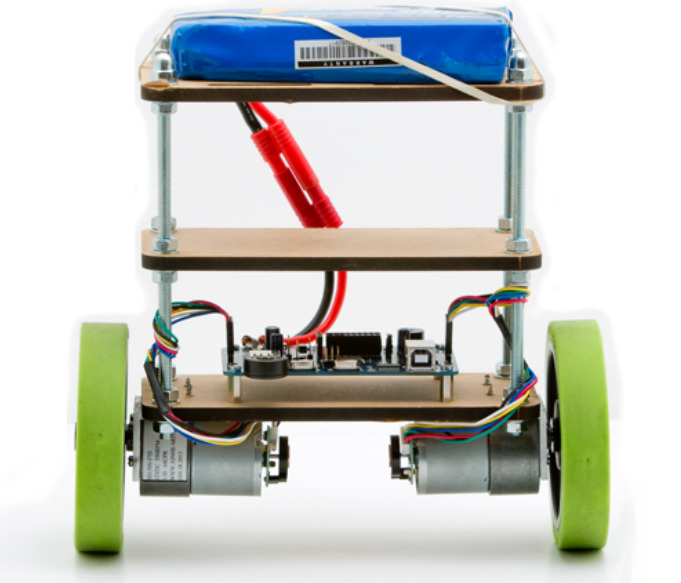
\includegraphics[width=0.7\columnwidth]{balanduino}
%	\caption{Example picture of the Balanduino robot. Place all figures at the top \texttt{[t]} (default) or bottom \texttt{[b]} (only if needed).}
%	\label{fig:gadget} % Should be placed after the caption!
%\end{figure}
%
%\subsection{Some Dummy Text}
%\kant[3]

\section{Implementation}
Here you describe how you implemented your learning or control design.

\section{Results}
If you need to use tables, Table~\ref{tab:extable} shows an example of how they can be typeset. For further details, see \cite{tablelatexwiki}.

\begin{table}[t]
	\centering
	\caption{Example table. Note that the caption goes on top. Place all tables at the top \texttt{[t]} (default) or bottom \texttt{[b]} (only if needed) of the page.}
	\label{tab:extable}
	\begin{tabular}{lcrrcrrcrr} % (l)eft, (r)ight and (c)enter indentation
		\toprule
        &
		\multicolumn{2}{c}{IAE [$\cdot 10^3$~s]} & &
		\multicolumn{2}{c}{$\text{var}(\tau^o)$ [s]} & &
		\multicolumn{2}{c}{$\tau^o_{max}$ [s]} \\[1mm]
		$M_C$            &  3     & 10  &~& 3     & 10    &~& 3    & 10 \\
        \midrule
		$C_{\text{orig}}$ & 8.23 & 8.34 &~& 0.695 & 0.745 &~& 5.68 & 6.27 \\
		$C_{\text{fb}}$ & 1.48 & 0.98 &~& 0.030 & 0.021 &~& 1.81 & 1.83 \\
		$C_{\text{ff}}$ & 1.23 & 1.43 &~& 0.026 & 0.034 &~& 1.56 & 1.65\\
        \bottomrule
	\end{tabular}
\end{table}

\subsection{Some Dummy Text}
\kant[4]

\section{Discussion}

Discuss the results and what you learned from the project.


% Prints cited references
\printbibliography


\end{document}
